\begin{frame}
  \frametitle{Topological Manifolds}
  \begin{defn}
    An $n$-dimensional topological mainfold is a topological space
    $M$ such that 
    \begin{enumerate}[(i)]
      \item For each $p \in M$, there exists a neighborhood 
        $p \in U \subseteq M$ and a homeomorphism 
        $\phi \colon U \to U' \subseteq \R^n$,
        where $U' = \phi(U)$ is an open subset of $\R^n$
      \item $M$ is second countable
      \item $M$ is Hausdorff
    \end{enumerate}
  \end{defn}
  We will recall topological notions later. 

  A topological space satisfying (i)
  is said to be locally Euclidean of dimension $n$.

  $(U, \phi)$ is a {\em chart} on $M$ near $p$.
\end{frame}
\begin{frame}
  \begin{example}
    Let $U'$ be an open subset of $\R^n$.
    Then $M = U'$ is an $n$-dimensional topological manifold.
    The identity map $\id \colon M \to U'$ is a chart near every $p \in M$.
  \end{example}
  \begin{example}
    Let $U' \subseteq \R^n$ be an open subset and let $f \colon U' \to \R^m$
    be a continuous function. The graph $\Gamma(f)$ is the subset of $\R^n
    \times \R^m$
    consisting of pairs $(x, f(x))$ for $x \in U'$. 
    The subspace $M = \Gamma(f)$ of $\R^n \times \R^m$
    is a topological manifold. The projection
    $\phi \colon \Gamma(f) \to U'$
    with $\phi(x, f(x)) = x$ is a chart near all $p \in M$.
    This is because its inverse $U' \to M$ taking $x$ to $(x, f(x))$
    is also continuous.
  \end{example}
\end{frame}
\begin{frame}
  \frametitle{Topological notions}
  \begin{defn}
    A topological space is a set $X$ together with a family $U$
    of subsets called the open sets.
    \begin{itemize}
      \item $\emptyset$ and $X$ are open
      \item All unions of open sets are open.
      \item Finite intersections of open sets are open.
    \end{itemize}
  \end{defn}
  A {\em neighborhood} of a point $p \in X$ is an open set containing $p$.

  \begin{defn}
    A family $\BB$
    of open sets in $X$ is a basis for the topology if: For each $p \in X$
    and each neighborhood $U$ of $p$, there exists a $B \in \BB$
    such that $p \in B \subseteq U$.
  \end{defn}

  Notice that if $\BB$ is a basis for the topology on $X$, then
  every open set in $X$ is a union of elements from $B$.
  \begin{example}
    $X = \R^n$, let $\BB$ be the collection of all open balls
    $B(p, \varepsilon)$ for $p \in \Q^n$ and $\varepsilon \in \Q$
    with $\varepsilon > 0$.
  \end{example}
\end{frame}
\begin{frame}
  \begin{defn}
    A topological space $X$ is second countable if there
    exists a countable basis for the topology.
  \end{defn}
  \begin{example}
    $X = \R^n$ with the bases of the previous example.
  \end{example}
  \begin{block}
    {Remark}
    If $X$ is second countable, then so is every subspace $A \subseteq X$.
    In particular every $A \subseteq \R^n$ is second countable.
  \end{block}
\end{frame}
\begin{frame}
  \begin{defn}
    A topological space $X$ is Hausdorff if for each pair of distinct
    points $p, q \in X$, there 
    exists neighborhoods $p \in U$ and $q \in V$ such that $U \cap V =
    \emptyset$.
  \end{defn}
  \begin{example}
    $\R^n$ is Hausdorff.
  \end{example}
  \begin{remark}
    If $X$ is Hausdorff, then so is every subspace $A \subseteq X$.
    In particular every $A \subseteq \R^n$ is Hausdorff.
  \end{remark}
\end{frame}
\begin{frame}
  \begin{defn}
    A function $f \colon X \to Y$ between topological spaces
    $X$ and $Y$ is {\em continuous} if the inverse image $f^{-1}(V)$ of
    every open set $V$ in $Y$ is open in $X$.
  \end{defn}
  \begin{defn}
    A continuous function is a {\em homeomorphism} if
    it is a bijection and the inverse function is 
    also continuous.
  \end{defn}
\end{frame}
\begin{frame}
  \frametitle{Compatible Charts}
  Let $M$ be a topological manifold with two charts $(U, \phi)$ 
  and $(V, \psi)$.

  \begin{center}
    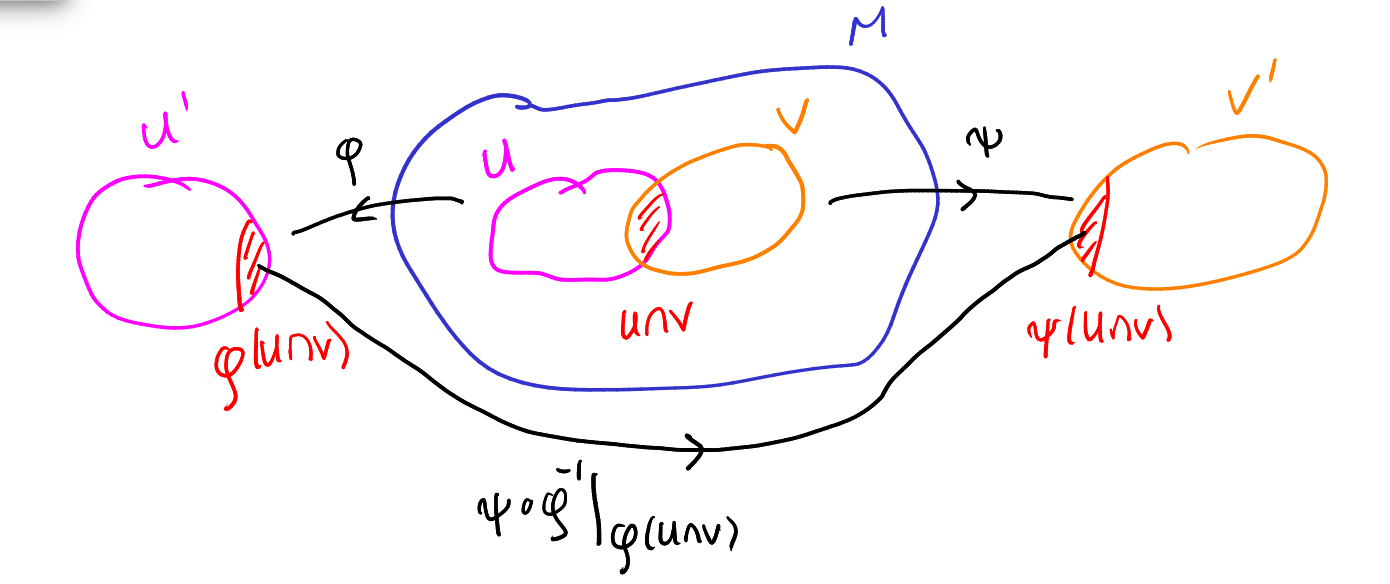
\includegraphics[width=0.7\textwidth]{figures/two_charts.png}
  \end{center}
  \begin{defn}
    Two charts $(U, \phi \colon U \to U')$ and
    $(V, \psi \colon V \to V')$ are 
    {\em $C^{\infty}$ compatible}
    if the two maps $\psi \circ \phi^{-1} \colon \phi(U \cap V) \to 
    \psi(U \cap V)$ and
    $\phi \circ \psi^{-1} \colon \psi(U \cap V) \to 
    \phi(U \cap V)$ are $C^{\infty}$.
  \end{defn}
\end{frame}

\begin{frame}
  \begin{defn}
    A $C^{\infty}$ atlas on a topological manifold $M$ is a collection of 
    charts $\{(U_\alpha, \phi_\alpha)\}$ such that $M = \cup U_\alpha$
    and the charts are pairwise compatible.
  \end{defn}
  \begin{example}[The unit circle (make illustration)]
    Let $M = S^1$ be the unit circle in $\R^2$.
    We define charts $(U_1, \phi_1)$ and $(U_2, \phi_2)$ on $M$:
    \begin{displaymath}
      U_1 = \{(x, y) \in S^1 \cond y > 0\} \quad 
      \text{and} \quad
      U_2 = \{(x, y) \in S^1 \cond x > 0\}
    \end{displaymath}
    Let $U_1' = (-1, 1)$ and also $U_2' = (-1, 1)$. Then $\phi_1 \colon
    U_1 \to U_1'$ defined by $\phi_1(x,y) = x$
    is a chart. This is because $U_1$ is the graph of the function
    $f \colon U_1' \to U_1$ with $f(t) = (t, \sqrt{1-t^2})$, and $f$
    is the inverse function of $\phi_1$. Also
    $\phi_2
    \colon U_2 \to U_2'$ defined by $\phi_2(x,y) = y$ is a chart.
    Now, $\phi_2 \circ \phi_1^{-1}  = \phi_2 \circ f$ is the 
    function $(\phi_2\circ) f(t) = \sqrt{1 - t^2}$.
    Since $\phi_1(U_1 \cap U_2) = (0, 1)$, this is a smooth
    function.
    Introducing two more charts in the negative quadrants we obtain a
    smooth atlas for the unit circle.
  \end{example}
\end{frame}
\begin{frame}
  \frametitle{Smooth Manifolds}
  \begin{defn}
    A $C^{\infty}$ atlas $\MM = \{(U_\alpha, \phi_\alpha)\}$
    is {\em maximal} if for any other $C^{\infty}$ atlas $\MM'$ on 
    $M$ such that $\MM \subseteq \MM'$, we have $\MM = \MM'$.
  \end{defn}
  \begin{defn}
    A smooth $n$-dimensional manifild is an $n$-dimensional
    topological manifold together with a maximal $\Cinfty$
    atlas.
  \end{defn}
  A maximal $\Cinfty$ atlas is also called a differentiable structure.
\end{frame}
\begin{frame}
  \begin{prop}
    Every $\Cinfty$ atlas on a topological mainfold is contained 
    in a unique maximal $Cinfty$ atlas.
  \end{prop}
  \begin{proof}
    Let $\{(U_\alpha, \phi_\alpha)\}$
    be a $\Cinfty$ atlas on $M$.
    Let $\MM$ be the set of all charts on $M$ that are compatible with
    all the charts 
    $(U_\alpha, \phi_\alpha)$.
    Note that if  $\MM$ is a $Cinfty$ atlas, then it is maximal.
    It remains to show that $\MM$ is a $\Cinfty$ atlas.
    Given charts $(U, \phi)$ and $(V,\psi)$ that are $Cinfty$
    compatible with all the charts
    $(U_\alpha, \phi_\alpha)$
    we need to show that 
    \begin{displaymath}
      \phi(U \cap V) \xto {\phi^{-1}} U \cap V \xto \psi \psi(U \cap V)
      \quad \text{is $\Cinfty$.}
    \end{displaymath}
    Let $p \in U \cap V$, and choose a chart 
    $(U_\alpha, \phi_\alpha)$
    with $p \in U_\alpha$.
    Then $p \in U \cap V \cap U_{\alpha}$, and on
    $U \cap V \cap U_{\alpha}$ we have 
    \begin{displaymath}
      \psi \circ \phi^{-1} = (\psi \circ \phi_{\alpha}^{-1}) \circ (\phi_\alpha
      \circ \phi^{-1})
    \end{displaymath}
    Since $(U, \phi)$ and $(V,\psi)$ that are $Cinfty$
    compatible with the chart
    $(U_\alpha, \phi_\alpha)$
    $\psi \circ \phi^{-1}$ is a composition of two smooth maps,
    so it is smooth.
  \end{proof}
  Consequence: When defining a $\Cinfty$ manifold it suffices to 
  specify only one $\Cinfty$ atlas.
\end{frame}
\begin{frame}
  \begin{example}
    Every atlas with only one chart is a $\Cinfty$ compatible atlas.
    In particular every open sbuset of $\R^n$ is a smooth manifold
    of dimension $n$.
  \end{example}
  \begin{example}
    We have indicated a smooth atlas on the circle $S^1$.
  \end{example}
  \begin{example}
    Every atlas with only one chart is a $\Cinfty$ compatible atlas.
    In particular, given an open subset $U \subseteq \R^n$ and a
    smooth function $f \colon U \to \R^m$, the graph $\Gamma(f)$
    is a smooth manifold.
  \end{example}
  Recall that $\Gamma(f) = \{(x, f(x)) \in \R^{n+m} \cond x \in U\}$ and that
  the projection $\phi \colon \Gamma(f) \to U$ taking $(x, y) \in \Gamma(f)$ to
  $x$ is a chart.
\end{frame}
\begin{frame}
  \begin{example}
    The general linear group $GL(n, \R)$ is the open subset of
    the vector space $\R^{n \times n}$ of $n \times n$-matrices consisting
    of matrices with nonzero determinant. Thus, it is a smooth manifold.
  \end{example}
  \begin{example}
    If $M$ and $N$ are smooth manifolds, then so is their product $M \times N$.
    In particular the cylinder $S^1 \times \R$ and the
    torus $S^1 \times S^1$ are manifolds.
  \end{example}

\end{frame}
